
%% bare_conf.tex
%% V1.3
%% 2007/01/11
%% by Michael Shell
%% See:
%% http://www.michaelshell.org/
%% for current contact information.
%%
%% This is a skeleton file demonstrating the use of IEEEtran.cls
%% (requires IEEEtran.cls version 1.7 or later) with an IEEE conference paper.
%%
%% Support sites:
%% http://www.michaelshell.org/tex/ieeetran/
%% http://www.ctan.org/tex-archive/macros/latex/contrib/IEEEtran/
%% and
%% http://www.ieee.org/

%%*************************************************************************
%% Legal Notice:
%% This code is offered as-is without any warranty either expressed or
%% implied; without even the implied warranty of MERCHANTABILITY or
%% FITNESS FOR A PARTICULAR PURPOSE! 
%% User assumes all risk.
%% In no event shall IEEE or any contributor to this code be liable for
%% any damages or losses, including, but not limited to, incidental,
%% consequential, or any other damages, resulting from the use or misuse
%% of any information contained here.
%%
%% All comments are the opinions of their respective authors and are not
%% necessarily endorsed by the IEEE.
%%
%% This work is distributed under the LaTeX Project Public License (LPPL)
%% ( http://www.latex-project.org/ ) version 1.3, and may be freely used,
%% distributed and modified. A copy of the LPPL, version 1.3, is included
%% in the base LaTeX documentation of all distributions of LaTeX released
%% 2003/12/01 or later.
%% Retain all contribution notices and credits.
%% ** Modified files should be clearly indicated as such, including  **
%% ** renaming them and changing author support contact information. **
%%
%% File list of work: IEEEtran.cls, IEEEtran_HOWTO.pdf, bare_adv.tex,
%%                    bare_conf.tex, bare_jrnl.tex, bare_jrnl_compsoc.tex
%%*************************************************************************

% *** Authors should verify (and, if needed, correct) their LaTeX system  ***
% *** with the testflow diagnostic prior to trusting their LaTeX platform ***
% *** with production work. IEEE's font choices can trigger bugs that do  ***
% *** not appear when using other class files.                            ***
% The testflow support page is at:
% http://www.michaelshell.org/tex/testflow/



% Note that the a4paper option is mainly intended so that authors in
% countries using A4 can easily print to A4 and see how their papers will
% look in print - the typesetting of the document will not typically be
% affected with changes in paper size (but the bottom and side margins will).
% Use the testflow package mentioned above to verify correct handling of
% both paper sizes by the user's LaTeX system.
%
% Also note that the "draftcls" or "draftclsnofoot", not "draft", option
% should be used if it is desired that the figures are to be displayed in
% draft mode.
%
\documentclass[conference]{IEEEtran}
\usepackage[]{blindtext, graphicx}
\usepackage[hidelinks]{hyperref}
\graphicspath{ {Figures/} }
\usepackage{tabularx}
\usepackage{longtable}
\usepackage{color}

% Add the compsoc option for Computer Society conferences.
%
% If IEEEtran.cls has not been installed into the LaTeX system files,
% manually specify the path to it like:
% \documentclass[conference]{../sty/IEEEtran}





% Some very useful LaTeX packages include:
% (uncomment the ones you want to load)


% *** MISC UTILITY PACKAGES ***
%
%\usepackage{ifpdf}
% Heiko Oberdiek's ifpdf.sty is very useful if you need conditional
% compilation based on whether the output is pdf or dvi.
% usage:
% \ifpdf
%   % pdf code
% \else
%   % dvi code
% \fi
% The latest version of ifpdf.sty can be obtained from:
% http://www.ctan.org/tex-archive/macros/latex/contrib/oberdiek/
% Also, note that IEEEtran.cls V1.7 and later provides a builtin
% \ifCLASSINFOpdf conditional that works the same way.
% When switching from latex to pdflatex and vice-versa, the compiler may
% have to be run twice to clear warning/error messages.






% *** CITATION PACKAGES ***
%
%\usepackage{cite}
% cite.sty was written by Donald Arseneau
% V1.6 and later of IEEEtran pre-defines the format of the cite.sty package
% \cite{} output to follow that of IEEE. Loading the cite package will
% result in citation numbers being automatically sorted and properly
% "compressed/ranged". e.g., [1], [9], [2], [7], [5], [6] without using
% cite.sty will become [1], [2], [5]--[7], [9] using cite.sty. cite.sty's
% \cite will automatically add leading space, if needed. Use cite.sty's
% noadjust option (cite.sty V3.8 and later) if you want to turn this off.
% cite.sty is already installed on most LaTeX systems. Be sure and use
% version 4.0 (2003-05-27) and later if using hyperref.sty. cite.sty does
% not currently provide for hyperlinked citations.
% The latest version can be obtained at:
% http://www.ctan.org/tex-archive/macros/latex/contrib/cite/
% The documentation is contained in the cite.sty file itself.






% *** GRAPHICS RELATED PACKAGES ***
%
\ifCLASSINFOpdf
  % \usepackage[pdftex]{graphicx}
  % declare the path(s) where your graphic files are
  % \graphicspath{{../pdf/}{../jpeg/}}
  % and their extensions so you won't have to specify these with
  % every instance of \includegraphics
  % \DeclareGraphicsExtensions{.pdf,.jpeg,.png}
\else
  % or other class option (dvipsone, dvipdf, if not using dvips). graphicx
  % will default to the driver specified in the system graphics.cfg if no
  % driver is specified.
  % \usepackage[dvips]{graphicx}
  % declare the path(s) where your graphic files are
  % \graphicspath{{../eps/}}
  % and their extensions so you won't have to specify these with
  % every instance of \includegraphics
  % \DeclareGraphicsExtensions{.eps}
\fi
% graphicx was written by David Carlisle and Sebastian Rahtz. It is
% required if you want graphics, photos, etc. graphicx.sty is already
% installed on most LaTeX systems. The latest version and documentation can
% be obtained at: 
% http://www.ctan.org/tex-archive/macros/latex/required/graphics/
% Another good source of documentation is "Using Imported Graphics in
% LaTeX2e" by Keith Reckdahl which can be found as epslatex.ps or
% epslatex.pdf at: http://www.ctan.org/tex-archive/info/
%
% latex, and pdflatex in dvi mode, support graphics in encapsulated
% postscript (.eps) format. pdflatex in pdf mode supports graphics
% in .pdf, .jpeg, .png and .mps (metapost) formats. Users should ensure
% that all non-photo figures use a vector format (.eps, .pdf, .mps) and
% not a bitmapped formats (.jpeg, .png). IEEE frowns on bitmapped formats
% which can result in "jaggedy"/blurry rendering of lines and letters as
% well as large increases in file sizes.
%
% You can find documentation about the pdfTeX application at:
% http://www.tug.org/applications/pdftex





% *** MATH PACKAGES ***
%
%\usepackage[cmex10]{amsmath}
% A popular package from the American Mathematical Society that provides
% many useful and powerful commands for dealing with mathematics. If using
% it, be sure to load this package with the cmex10 option to ensure that
% only type 1 fonts will utilized at all point sizes. Without this option,
% it is possible that some math symbols, particularly those within
% footnotes, will be rendered in bitmap form which will result in a
% document that can not be IEEE Xplore compliant!
%
% Also, note that the amsmath package sets \interdisplaylinepenalty to 10000
% thus preventing page breaks from occurring within multiline equations. Use:
%\interdisplaylinepenalty=2500
% after loading amsmath to restore such page breaks as IEEEtran.cls normally
% does. amsmath.sty is already installed on most LaTeX systems. The latest
% version and documentation can be obtained at:
% http://www.ctan.org/tex-archive/macros/latex/required/amslatex/math/





% *** SPECIALIZED LIST PACKAGES ***
%
%\usepackage{algorithmic}
% algorithmic.sty was written by Peter Williams and Rogerio Brito.
% This package provides an algorithmic environment fo describing algorithms.
% You can use the algorithmic environment in-text or within a figure
% environment to provide for a floating algorithm. Do NOT use the algorithm
% floating environment provided by algorithm.sty (by the same authors) or
% algorithm2e.sty (by Christophe Fiorio) as IEEE does not use dedicated
% algorithm float types and packages that provide these will not provide
% correct IEEE style captions. The latest version and documentation of
% algorithmic.sty can be obtained at:
% http://www.ctan.org/tex-archive/macros/latex/contrib/algorithms/
% There is also a support site at:
% http://algorithms.berlios.de/index.html
% Also of interest may be the (relatively newer and more customizable)
% algorithmicx.sty package by Szasz Janos:
% http://www.ctan.org/tex-archive/macros/latex/contrib/algorithmicx/




% *** ALIGNMENT PACKAGES ***
%
%\usepackage{array}
% Frank Mittelbach's and David Carlisle's array.sty patches and improves
% the standard LaTeX2e array and tabular environments to provide better
% appearance and additional user controls. As the default LaTeX2e table
% generation code is lacking to the point of almost being broken with
% respect to the quality of the end results, all users are strongly
% advised to use an enhanced (at the very least that provided by array.sty)
% set of table tools. array.sty is already installed on most systems. The
% latest version and documentation can be obtained at:
% http://www.ctan.org/tex-archive/macros/latex/required/tools/


%\usepackage{mdwmath}
%\usepackage{mdwtab}
% Also highly recommended is Mark Wooding's extremely powerful MDW tools,
% especially mdwmath.sty and mdwtab.sty which are used to format equations
% and tables, respectively. The MDWtools set is already installed on most
% LaTeX systems. The lastest version and documentation is available at:
% http://www.ctan.org/tex-archive/macros/latex/contrib/mdwtools/


% IEEEtran contains the IEEEeqnarray family of commands that can be used to
% generate multiline equations as well as matrices, tables, etc., of high
% quality.


%\usepackage{eqparbox}
% Also of notable interest is Scott Pakin's eqparbox package for creating
% (automatically sized) equal width boxes - aka "natural width parboxes".
% Available at:
% http://www.ctan.org/tex-archive/macros/latex/contrib/eqparbox/





% *** SUBFIGURE PACKAGES ***
%\usepackage[tight,footnotesize]{subfigure}
% subfigure.sty was written by Steven Douglas Cochran. This package makes it
% easy to put subfigures in your figures. e.g., "Figure 1a and 1b". For IEEE
% work, it is a good idea to load it with the tight package option to reduce
% the amount of white space around the subfigures. subfigure.sty is already
% installed on most LaTeX systems. The latest version and documentation can
% be obtained at:
% http://www.ctan.org/tex-archive/obsolete/macros/latex/contrib/subfigure/
% subfigure.sty has been superceeded by subfig.sty.



%\usepackage[caption=false]{caption}
%\usepackage[font=footnotesize]{subfig}
% subfig.sty, also written by Steven Douglas Cochran, is the modern
% replacement for subfigure.sty. However, subfig.sty requires and
% automatically loads Axel Sommerfeldt's caption.sty which will override
% IEEEtran.cls handling of captions and this will result in nonIEEE style
% figure/table captions. To prevent this problem, be sure and preload
% caption.sty with its "caption=false" package option. This is will preserve
% IEEEtran.cls handing of captions. Version 1.3 (2005/06/28) and later 
% (recommended due to many improvements over 1.2) of subfig.sty supports
% the caption=false option directly:
%\usepackage[caption=false,font=footnotesize]{subfig}
%
% The latest version and documentation can be obtained at:
% http://www.ctan.org/tex-archive/macros/latex/contrib/subfig/
% The latest version and documentation of caption.sty can be obtained at:
% http://www.ctan.org/tex-archive/macros/latex/contrib/caption/




% *** FLOAT PACKAGES ***
%
%\usepackage{fixltx2e}
% fixltx2e, the successor to the earlier fix2col.sty, was written by
% Frank Mittelbach and David Carlisle. This package corrects a few problems
% in the LaTeX2e kernel, the most notable of which is that in current
% LaTeX2e releases, the ordering of single and double column floats is not
% guaranteed to be preserved. Thus, an unpatched LaTeX2e can allow a
% single column figure to be placed prior to an earlier double column
% figure. The latest version and documentation can be found at:
% http://www.ctan.org/tex-archive/macros/latex/base/



%\usepackage{stfloats}
% stfloats.sty was written by Sigitas Tolusis. This package gives LaTeX2e
% the ability to do double column floats at the bottom of the page as well
% as the top. (e.g., "\begin{figure*}[!b]" is not normally possible in
% LaTeX2e). It also provides a command:
%\fnbelowfloat
% to enable the placement of footnotes below bottom floats (the standard
% LaTeX2e kernel puts them above bottom floats). This is an invasive package
% which rewrites many portions of the LaTeX2e float routines. It may not work
% with other packages that modify the LaTeX2e float routines. The latest
% version and documentation can be obtained at:
% http://www.ctan.org/tex-archive/macros/latex/contrib/sttools/
% Documentation is contained in the stfloats.sty comments as well as in the
% presfull.pdf file. Do not use the stfloats baselinefloat ability as IEEE
% does not allow \baselineskip to stretch. Authors submitting work to the
% IEEE should note that IEEE rarely uses double column equations and
% that authors should try to avoid such use. Do not be tempted to use the
% cuted.sty or midfloat.sty packages (also by Sigitas Tolusis) as IEEE does
% not format its papers in such ways.





% *** PDF, URL AND HYPERLINK PACKAGES ***
%
%\usepackage{url}
% url.sty was written by Donald Arseneau. It provides better support for
% handling and breaking URLs. url.sty is already installed on most LaTeX
% systems. The latest version can be obtained at:
% http://www.ctan.org/tex-archive/macros/latex/contrib/misc/
% Read the url.sty source comments for usage information. Basically,
% \url{my_url_here}.





% *** Do not adjust lengths that control margins, column widths, etc. ***
% *** Do not use packages that alter fonts (such as pslatex).         ***
% There should be no need to do such things with IEEEtran.cls V1.6 and later.
% (Unless specifically asked to do so by the journal or conference you plan
% to submit to, of course. )


% correct bad hyphenation here
\hyphenation{op-tical net-works semi-conduc-tor}


\begin{document}
%
% paper title
% can use linebreaks \\ within to get better formatting as desired
\title{Stock forecasting algorithms and their usage}


% author names and affiliations
% use a multiple column layout for up to three different
% affiliations
\author{\IEEEauthorblockN{Marc Misoch}
\IEEEauthorblockA{Institute of Computer Science\\University of Applied Science\\
Mannheim, Germany\\
Email: marc.misoch@stud.hs-mannheim.de}
\and
\IEEEauthorblockN{David Marquant}
\IEEEauthorblockA{Institute of Computer Science\\University of Applied Science\\
Mannheim, Germany\\
Email: david.marquant@stud.hs-mannheim.de}
}

% conference papers do not typically use \thanks and this command
% is locked out in conference mode. If really needed, such as for
% the acknowledgment of grants, issue a \IEEEoverridecommandlockouts
% after \documentclass

% for over three affiliations, or if they all won't fit within the width
% of the page, use this alternative format:
% 
%\author{\IEEEauthorblockN{Michael Shell\IEEEauthorrefmark{1},
%Homer Simpson\IEEEauthorrefmark{2},
%James Kirk\IEEEauthorrefmark{3}, 
%Montgomery Scott\IEEEauthorrefmark{3} and
%Eldon Tyrell\IEEEauthorrefmark{4}}
%\IEEEauthorblockA{\IEEEauthorrefmark{1}School of Electrical and Computer Engineering\\
%Georgia Institute of Technology,
%Atlanta, Georgia 30332--0250\\ Email: see http://www.michaelshell.org/contact.html}
%\IEEEauthorblockA{\IEEEauthorrefmark{2}Twentieth Century Fox, Springfield, USA\\
%Email: homer@thesimpsons.com}
%\IEEEauthorblockA{\IEEEauthorrefmark{3}Starfleet Academy, San Francisco, California 96678-2391\\
%Telephone: (800) 555--1212, Fax: (888) 555--1212}
%\IEEEauthorblockA{\IEEEauthorrefmark{4}Tyrell Inc., 123 Replicant Street, Los Angeles, California 90210--4321}}




% use for special paper notices
%\IEEEspecialpapernotice{(Invited Paper)}




% make the title area
\maketitle


\begin{abstract}
%\boldmath
In this paper, we propose several methods to predict future stock prices. There are
a lot of algorithms out there but some are more reliable than others. As expected,
in most cases the general rule: \textit{"the more complex, the better the prediction" } is true.
However there are some relatively easy algorithms than can predict the stock prices of the future quite well.
We are going to present and analyse some of these algorithms and take a deeper look into them.
Just to make this clear, there is not a single algorithm, than can predict the future of a 
stock 100\% correctly. The relationships of the global stock market are to complex to bring them down in a 
single computer program. We will show the experimental results we got with several algorithms and compare them.
Also we will take a short look into investment strategies based on these forecasts and take a look at the results.
\end{abstract}
% IEEEtran.cls defaults to using nonbold math in the Abstract.
% This preserves the distinction between vectors and scalars. However,
% if the journal you are submitting to favors bold math in the abstract,
% then you can use LaTeX's standard command \boldmath at the very start
% of the abstract to achieve this. Many IEEE journals frown on math
% in the abstract anyway.

% Note that keywords are not normally used for peerreview papers.
\begin{IEEEkeywords}
stock, forecast, prediction, paper, algorithms, neuronal-network.
\end{IEEEkeywords}






% For peer review papers, you can put extra information on the cover
% page as needed:
% \ifCLASSOPTIONpeerreview
% \begin{center} \bfseries EDICS Category: 3-BBND \end{center}
% \fi
%
% For peerreview papers, this IEEEtran command inserts a page break and
% creates the second title. It will be ignored for other modes.
\IEEEpeerreviewmaketitle



\section{Introduction}
\label{introduction}
\subsection{Introduction to stock forecasting}

There is a huge variety of methods that are used in forecasting stock prices. Many of the algorithms that have been made up just use structured data like tables with historic stock quotes in it. The aim of all these algorithms is to maximize the profit while keeping the risk as low as possible.

Since the stock market is global, there are many relationships between stocks. Some of them are paired with others so if the price of one stock goes down, the other stock will follow this trend.
Stocks are also influenced by numerous factors and these factors also have relationships between each other. This leads us to the thought, that a good stock prediction has to consider more than just past stock prices. However it is still possible to make reasonably good predictions based on just previous prices.

One very important thing that to observe is influence of international newscasts. If the global economy, or even the economy of a single country is experiencing a financial crisis, the stock market will follow that trend. But those trends are most likely to be relatively slow and easy to predict even looking at the stock prices itself. What is more dangerous are catastrophes. After a catastrophe there is often a low point on the stock market. This low point comes so fast, that only algorithms that observe the news have a chance to prevent huge losses.

Another to note is, that we did all our tests on historic data of the stock market. Even if we \textit{bought} a stock at some specific point of time, we did not really buy this stock on the real market. So our tests did not affect the stock market at all. Because buying and selling stocks on the market while testing, would always affect the received results.

\subsection{Motivation}

In this paper we are going to compare some algorithms and their functionality. The main goal of these algorithms is, to predict a rise or fall in the price before the actual rise or fall happens. It is very important to find some kind of pattern in the stock prices of the past to do a accurate prediction of the future prices. We also like to share some of our experimental results we had with the algorithms. We only used algorithms that do not take global news in account because we wanted to see, how good the algorithms were in an isolated environment analysing past prices only. We decided to do it that way, because the algorithms themselves should work properly and examining news would be an easy addition to these working algorithms.

The main goal of the project was, to find a good working stock forecast algorithm to predict future stock trends. Later in this paper, we will introduce parameters and variables, that give the best results combined with our algorithms.

\subsection{Document overview}
Section \ref{essentials} briefly covers the background information needed for the reader to understand the most important points about our project.

Section \ref{algorithm} describes the algorithms used in more detail. 

Chapter \ref{results} is about the test-results received using the algorithms described in chapter \ref{algorithm}. All algorithms were tested with different inputs and parameters.

In section \ref{conclusion} the results are interpreted and we propose how our algorithms can be improved to be successful in the real stock market.

In chapter \ref{futurework} some thing extensions to our algorithms are given, which could be done in future.


\section{Essentials}
\label{essentials}

We investigated algorithms that bring good results with time series analysis. The computer programs we implemented were specialized  making a good prediction only looking at one single stock and its trend. These algorithms were tested on real stock data we fetched from the yahoo finance API. 

We used yahoo finance because it gives easy access to numerous stocks and their historical prices. The API yahoo grants is pretty simple. The only thing you have to do to download the data you need is, preparing a link so it fits your needs. For example the url -

\textit{\url{http://real-chart.finance.yahoo.com/table.csv?s=IBM&a=00&b=2&c=1962&d=04&e=21&f=2015&g=d&ignore=.csv}}
\\
\\
- provides the data in a csv-file. The stock that this link is going to download is IBM (International Business Machines Corporation). It is also possible to adjust the timespan and format of the data. 
This method of getting historical stock market data is pretty easy to implement in various programming languages. It is also possible to download the csv-file to your computer with this link.

After acquiring the necessary data, we started implementing the algorithms that we thought of. 

\section{Algorithms}
\label{algorithm}

We implemented three different algorithms to predict stock prices and maximise the outcome. All three of them only consider one stock at a time and do not take any global news or trends in account. In this section describes the algorithms used in detail

\subsection{Algorithm using the latest trend}

With this algorithm we wanted to make a precise prediction on the stock market. It analyses the closing prices of a specific stock and gives a forecast how the price will develop. We also wanted the algorithm to be able to predict not only the price for the next day, but for the next few days. In section \ref{results} we will demonstrate that we were able to do a good prediction even 4 days in the future. But it must be said that the more in the future the prediction is, the bigger the gap between the real prices and the prediction.

The algorithm itself uses only the last few days of a stock. The number of days used for this algorithm is not static. The amount of days that give the best result may vary for different stocks. Nevertheless if the number of days stays within a specific range, the results are pretty accurate.
\\
\\
\[ M = \sum_{n=0}^D C_{n+1} - C_{n} \]
\[ prediction = \frac{M}{D}\]
\[ stock_{predicted} = stock_{today} + prediction\]
\\
Where D is the number of days the prediction is based on and C is the closing price of the nth day. After you calculated the prediction, the only thing that is left to do, is adding the prediction to the actual stock price. The predicted stock price here is for the next day only. 

To get the prediction for the day after that, do this calculation again but take the predicted stock into account.It is possible to do this over and over again for as many days in the future as you would like. Though it is not meaningful for more than a few days because the prediction gets more and more unreliable. For detailed results an the amount of days that are rational, see chapter \ref{results} on page 
\pageref{results}.

\subsection{Algorithm using long term moving average}

This algorithm is based on analysing the moving average of a stock. It does not make a prediction about the precise prise of a stock the next day. The only thing it does, is giving an advice when to buy a stock and when to sell it. If you follow the advices of this algorithm, it is possible to have a positive outcome even if the trend of a stock is overall going down.

The first thing we had to do was calculating the moving average of a stock. This can be computed as below-
\\
\\
$ MA_{n} =  \frac{C_{D} + C_{D-1} + ... + C_{D-(n-1)}}{n} $
\\
\\
Where C is the closing price of a stock on a specific day D.

Now we need to calculate MA$ _{50} $\footnote{Moving average of the last 50 days} and MA$ _{200} $\footnote{Moving average of the last 200 days} of a specific stock we want to invest in.

If the condition MA$ _{50} >$  MA$ _{200} $ is fulfilled the algorithms gives the advice to buy the stock on this day. After the stock has been bought, the algorithm checks every day if the requirement is still met. As soon as MA$ _{50} <$  MA$ _{200} $ the algorithm recommends to sell the stock. This algorithm seems to be very simple but it is worth noticing, that the outcome was pretty solid in the test we made. For detailed results, see chapter \ref{results} on page  \pageref{results}.



\subsection{Algorithm using supervised learning techniques}

In forecasting future stock trends it is common to not use the stock prices itself. Instead other values based on the stock prices are first calculated and then used as predictor variables for the learning process. One possible value is the daily return which is:
\\
\\
$Return_i = \frac{Close_i - Close_{i-1}}{Close_{i-1}}$
\\
\\
For this algorithm three different techniques are used to learn the model of the stock trends. Those are Logistic Regression, Linear Discriminant Analysis and Quadratic Discriminant Analysis. To test them the returns of the past two days are used as predictor variables. 

Through Logistic Regression the probability of a following day being categorized as "Up" or "Down" is modelled. The function used for logistic regression is the following:
\\
\\
$p(Y = U | L_1, L_2) = \frac{e^{\beta_0 + \beta_1 L_1 + \beta_2 L_2}}{1 + e^{\beta_0 + \beta_1 L_1 + \beta_2 L_2}}$
\\
\\
Where $p(Y = U)$ is the probability that the next day's stock price is increasing. $L_1$ and $L_2$ are the lagged returns of the past two days.

Linear and Quadratic Discriminant Analysis both treat their predictor variables independently at first and combine them later using Bayes' theorem.
\section{Results}
\label{results}

This chapter is about the results we had with each algorithm individually. We will also discuss which parameters gave the best and worst results and why that happened. 

\subsection{Algorithm using the latest trend}

How this algorithm works in detail is described in section \ref{algorithm}. This algorithm is all about predicting the exact price of a stock for the next days. With this algorithm we tried to predict if a stock would go down or up on the next day. We also tried to predict more than just one day in the future. Later in this chapter we will show how good our predictions were on the first and on the nth day in the future. It is understandable that, the more you go into the future, the more unreliable the predictions become. 

To get better and more reliable results, we did not test this method on single stocks. We wanted to get a big amount of predictions and see whether they were good. Because if you only predict one single price it is not really significant, but if you predict many prices and take the average of these predictions you get meaningful results. That is why we took 150 stocks for our algorithm to predict. We tested 3 sets of data with 150 stocks each.

Also a very important thing is the amount of days the algorithm uses to make its prediction. We got the best results using something in the span of 10-15 past days. If you use more than 15 days, it does not really take the latest trend into account and if you use less than 10 days the timespan to get a good prediction is to short.

\begin{center}
\begin{tabularx}{0.49\textwidth}{|X|X|X|X|}
\hline
Days in the future & Set 1 & Set 2 & Set 3\\
\hline
\hline
Day 1. & 0.043 \$ & 0.012 \$ & 0.028 \$\\
\hline
Day 2. & 0.049 \$ & 0.010 \$ & 0.033 \$\\
\hline
Day 3. & 0.059 \$ & 0.013 \$ & 0.041 \$\\
\hline
Day 4. & 0.089 \$ & 0.017 \$ & 0.038 \$\\
\hline
Day 5. & 0.092 \$ & 0.024 \$ & 0.049 \$\\
\hline
Day 6 & 0.126 \$ & 0.035 \$ & 0.062 \$\\
\hline
\hline
Day 15. & 1.740 \$ & 0.092 \$ & 0.107 \$\\
\hline

\end{tabularx}
\\[5pt]
Table 1. Difference between prediction and real data
\end{center}

You can see in this table, that the prediction for the first 3-4 days is relatively accurate. However the time after that the difference between prediction and real data gets bigger. Nevertheless in the first 6 days its still in an acceptable scope. But there are relatively big differences between the sets. These differences come with the fact that, if a stock is going smooth out prediction algorithm is pretty accurate. The algorithm is not good on predicting big price drops so if that happens the prediction gets pretty inaccurate. We suppose that in our first test set, there were more stocks with price spices than in the other to sets. That explains, that the predictions of the first set are not as accurate as the other two sets. So we consider our algorithm to be pretty accurate if the stock market goes smooth and has no big spikes because of some external reason. A span of a few cents in a prediction of 150 stocks is pretty accurate in our opinion.

\subsection{Algorithm using long term moving average}

As described in Chapter \ref{algorithm} this algorithm uses two different MA's to make a good prediction when to buy and when to sell a stock. It is not an algorithm to predict an exact price but rather to make profit without knowing the exact price the stock is going to have the next days.

\begin{figure}[!h]
  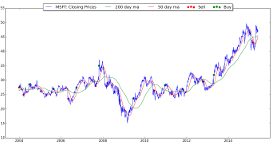
\includegraphics{MSFT_MA}
  \caption{Moving Average of MSFT (Microsoft Corporation)}
  \label{fig:MSFT_MA}
\end{figure}

 In Figure \ref{fig:MSFT_MA} you can see the development the stock of Microsoft Corporation\texttrademark made, in the last 11 years. If you look closely, there is also a red and green line in this Figure. The green line is the MA of the last 200 days of every point in this graph. The  red line marks the MA of the last 50 days. Now as described in section \ref{algorithm}, we used these two things to figure out when to buy and when to sell a stock.

We now take a closer look at a single passage of the stock to explain our approach in more detail.

\begin{figure}[!h]
  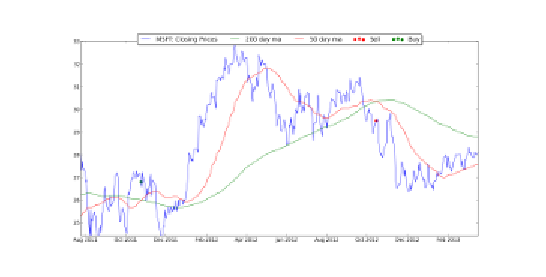
\includegraphics{MSFT_Zoomed}
  \caption{MSFT stock zoomed}
  \label{fig:MSFT_Z}
\end{figure}

Figure \ref{fig:MSFT_Z} shows only a small segment of the stocks development. You can see now, that the real stock price (blue line) is way different to both of the MA's. If you look closely, there is a red and a green dot on the stock price. This dots mark the spots, where the 200 day MA and the 50 day MA cross each other. Every time this happens, it is best to either sell of buy the stock. If the dot is green, the algorithms says, that now is the right time to buy the stock for the current price. And if it is red, the best thing is to sell the stock. The dots are on the blue line, because it marks the real price of the stock at this point of time. With this algorithm, we had good results as shown in the table below. We only investigated the last 1000 days of a stock for our test because we thought this was enough data to work with. So we tested our algorithm and bought and sold stocks based on the algorithm. In the first column of the table below you see the stocks we tested the algorithm with. In the second column, we wrote down, how much profit we made buying and selling only \textbf{one} instance of the stock. Just to make this clear, if you would by two instances of the stock you would make double the profit of loss we made. Remember that this are only examples, this results are not generalizable in any way. But we did not only do test with single stocks as they are not to meaningful. That is why we generated 100 random stocks and used our algorithm on all of them at the same time to get more significant results.

\begin{center}
\begin{tabularx}{0.49\textwidth}{|X|X|}
\hline
Stock(s) used & Outcome\\
\hline
\hline
MSFT\footnote{Microsoft Corporation\texttrademark} & 13.39 \$\\
\hline
MCD\footnote{McDonald's Corp\texttrademark} & 2.71 \$\\
\hline
YHOO\footnote{Yahoo! Inc.\texttrademark} & 20.05 \$\\
\hline

NVDA\footnote{NVIDIA Corporation\texttrademark} & \textcolor{red}{-13.70 \$}\\
\hline
INTC\footnote{Intel Corporation\texttrademark} & 5.70 \$\\
\hline
AMZN\footnote{Amazon.com Inc.\texttrademark} & 128.87 \$\\
\hline
\hline
Random combination 1. & 34.53 \$\\
\hline
Random combination 2. &\textcolor{red}{-17.32 \$}\\
\hline
Random combination 3. & 56.94 \$\\
\hline
Random combination 4. & 15.74 \$\\
\hline
\end{tabularx}
\\[5pt]
Table 2. Results of LTMA
\end{center}

As you can see in the table, our results with this algorithm were pretty good. While the single stock outcome is not very expressive, the results of the random combination of 100 stocks is also fine. If we only take the combinations of stocks into account, we made a total profit of \textbf{89.89 \$}. However this are only our test results with the amount of stocks we tested in a special period of time. Even with these test results it is not ensured, that our algorithm would always or even most of the time make profit.

\subsection{Algorithm using supervised learning techniques}

The algorithms were implemented in python utilizing the scikit-learn library.

The following table shows the results of applying different machine learning techniques to stock data. All used methods achieve similar results. The accuracy of the prediction is barely higher than the probability of a coin flip. But none of the cases do have a prediction accuracy below 50\%. The algorithm, as it is, should not be used without further improvements and refinement. 
\\
\begin{center}
\begin{tabularx}{0.5\textwidth}{|X|X|X|X|X|X|}
\hline
{} &     
\^{}AXJO\footnote{Australia ASX-200} &     
\^{}FCHI\footnote{Paris CAC 40} &     
\^{}FTSE\footnote{London FTSE-100} &    
\^{}GDAXI\footnote{Frankfurt DAX} & 
\^{}IXIC\footnote{NASDAQ Composite}\\
\hline
LDA &  0.501 &  0.541 &  0.527 &  0.555 & 0.571\\
LR  &  0.501 &  0.541 &  0.527 &  0.555 & 0.571\\
QDA &  0.541 &  0.513 &  0.519 &  0.539 & 0.575\\
\hline
\end{tabularx}
\\[5pt]
Table 3. Results of Supervised Learning Algorithms
\end{center}

% needed in second column of first page if using \IEEEpubid
%\IEEEpubidadjcol

% An example of a floating figure using the graphicx package.
% Note that \label must occur AFTER (or within) \caption.
% For figures, \caption should occur after the \includegraphics.
% Note that IEEEtran v1.7 and later has special internal code that
% is designed to preserve the operation of \label within \caption
% even when the captionsoff option is in effect. However, because
% of issues like this, it may be the safest practice to put all your
% \label just after \caption rather than within \caption{}.
%
% Reminder: the "draftcls" or "draftclsnofoot", not "draft", class
% option should be used if it is desired that the figures are to be
% displayed while in draft mode.
%
%\begin{figure}[!t]
%\centering
%\includegraphics[width=2.5in]{myfigure}
% where an .eps filename suffix will be assumed under latex, 
% and a .pdf suffix will be assumed for pdflatex; or what has been declared
% via \DeclareGraphicsExtensions.
%\caption{Simulation Results}
%\label{fig_sim}
%\end{figure}

% Note that IEEE typically puts floats only at the top, even when this
% results in a large percentage of a column being occupied by floats.


% An example of a double column floating figure using two subfigures.
% (The subfig.sty package must be loaded for this to work.)
% The subfigure \label commands are set within each subfloat command, the
% \label for the overall figure must come after \caption.
% \hfil must be used as a separator to get equal spacing.
% The subfigure.sty package works much the same way, except \subfigure is
% used instead of \subfloat.
%
%\begin{figure*}[!t]
%\centerline{\subfloat[Case I]\includegraphics[width=2.5in]{subfigcase1}%
%\label{fig_first_case}}
%\hfil
%\subfloat[Case II]{\includegraphics[width=2.5in]{subfigcase2}%
%\label{fig_second_case}}}
%\caption{Simulation results}
%\label{fig_sim}
%\end{figure*}
%
% Note that often IEEE papers with subfigures do not employ subfigure
% captions (using the optional argument to \subfloat), but instead will
% reference/describe all of them (a), (b), etc., within the main caption.


% An example of a floating table. Note that, for IEEE style tables, the 
% \caption command should come BEFORE the table. Table text will default to
% \footnotesize as IEEE normally uses this smaller font for tables.
% The \label must come after \caption as always.
%
%\begin{table}[!t]
%% increase table row spacing, adjust to taste
%\renewcommand{\arraystretch}{1.3}
% if using array.sty, it might be a good idea to tweak the value of
% \extrarowheight as needed to properly center the text within the cells
%\caption{An Example of a Table}
%\label{table_example}
%\centering
%% Some packages, such as MDW tools, offer better commands for making tables
%% than the plain LaTeX2e tabular which is used here.
%\begin{tabular}{|c||c|}
%\hline
%One & Two\\
%\hline
%Three & Four\\
%\hline
%\end{tabular}
%\end{table}


% Note that IEEE does not put floats in the very first column - or typically
% anywhere on the first page for that matter. Also, in-text middle ("here")
% positioning is not used. Most IEEE journals use top floats exclusively.
% Note that, LaTeX2e, unlike IEEE journals, places footnotes above bottom
% floats. This can be corrected via the \fnbelowfloat command of the
% stfloats package.



\section{Conclusion}
\label{conclusion}

The conclusion of this paper is, that you can get pretty good results in forecasting stock prices and try to get profit out of the stock market even with algorithms that do not consider the global news. However the stock market is pretty fragile and fast-paced, so while you are trying to make profit, it is always a possibility that the exact opposite happens. But with the right algorithms it can be worth the risk of investing into the market. 

\section{Future Work}
\label{futurework}

We implemented good working algorithms that can predict the stock price. But if these algorithms would take the global news into account there prediction could be better. With our algorithms we can never have a perfect result because if something global happens that affects the stock market, our algorithms are not fast enough to react and sell all stocks we bought. So the addition of a newscrawler would be a good idea for future work because it would help making the algorithms even more reliable in unforeseeable circumstances.



% if have a single appendix:
%\appendix[Proof of the Zonklar Equations]
% or
%\appendix  % for no appendix heading
% do not use \section anymore after \appendix, only \section*
% is possibly needed

% use appendices with more than one appendix
% then use \section to start each appendix
% you must declare a \section before using any
% \subsection or using \label (\appendices by itself
% starts a section numbered zero.)
%


\appendix
\section*{list of abbreviations}
MA - Moving average
\\
LTMA - Long term moving average Algorithm
\\
LTA - Latest trend algorithm
\\
LR - Logistic Regression
\\
LDA - Linear Discriminant Analysis
\\
QDA - Quadratic Discriminant Analysis

% use section* for acknowledgement
\section*{Acknowledgment}

The authors would like to thank Prof. Dr. Joern Fischer for his help and support while researching in this subject




% Can use something like this to put references on a page
% by themselves when using endfloat and the captionsoff option.
\ifCLASSOPTIONcaptionsoff
  \newpage
\fi



% trigger a \newpage just before the given reference
% number - used to balance the columns on the last page
% adjust value as needed - may need to be readjusted if
% the document is modified later
%\IEEEtriggeratref{8}
% The "triggered" command can be changed if desired:
%\IEEEtriggercmd{\enlargethispage{-5in}}

% references section

% can use a bibliography generated by BibTeX as a .bbl file
% BibTeX documentation can be easily obtained at:
% http://www.ctan.org/tex-archive/biblio/bibtex/contrib/doc/
% The IEEEtran BibTeX style support page is at:
% http://www.michaelshell.org/tex/ieeetran/bibtex/
%\bibliographystyle{IEEEtran}
% argument is your BibTeX string definitions and bibliography database(s)
%\bibliography{IEEEabrv,../bib/paper}
%
% <OR> manually copy in the resultant .bbl file
% set second argument of \begin to the number of references
% (used to reserve space for the reference number labels box)
\begin{thebibliography}{1}

\bibitem{IEEEhowto:kopka}
H.~Kopka and P.~W. Daly, \emph{A Guide to \LaTeX}, 3rd~ed.\hskip 1em plus
  0.5em minus 0.4em\relax Harlow, England: Addison-Wesley, 1999.
  
  \bibitem{Khaled}
  Stock price prediction using genetic algorithms and evolution
strategies
Ganesh Bonde, Rasheed Khaled

\bibitem{zhang}
Stock Market Forecasting Using Machine Learning Algorithms
Shunrong Shen, Haomiao Jiang, Tongda Zhang

\bibitem{Tang}
Stock Price Forecasting by Combining News Mining and Time Series Analysis
Xiangyu Tang, Chunyu Yang, Jie Zhou

\end{thebibliography}

% biography section
% 
% If you have an EPS/PDF photo (graphicx package needed) extra braces are
% needed around the contents of the optional argument to biography to prevent
% the LaTeX parser from getting confused when it sees the complicated
% \includegraphics command within an optional argument. (You could create
% your own custom macro containing the \includegraphics command to make things
% simpler here.)
%\begin{biography}[{\includegraphics[width=1in,height=1.25in,clip,keepaspectratio]{mshell}}]{Michael Shell}
% or if you just want to reserve a space for a photo:

%\begin{IEEEbiography}[{\includegraphics[width=1in,height=1.25in,clip,keepaspectratio]{picture}}]{John Doe}
%\blindtext
%\end{IEEEbiography}

% You can push biographies down or up by placing
% a \vfill before or after them. The appropriate
% use of \vfill depends on what kind of text is
% on the last page and whether or not the columns
% are being equalized.

%\vfill

% Can be used to pull up biographies so that the bottom of the last one
% is flush with the other column.
%\enlargethispage{-5in}

% that's all folks
\end{document}


